\documentclass[a4paper, fontsize = 14pt]{article}
\usepackage{hyperref}
\usepackage[warn]{mathtext}
\usepackage[english,russian]{babel}
\usepackage[utf8x]{inputenc} 
 
%математика
\usepackage[mathscr]{eucal}
\usepackage{amsmath,amsfonts,amssymb,amsthm,mathtools}
\usepackage{icomma}
\usepackage{wasysym}
\usepackage{mathrsfs}
\usepackage[italicdiff]{physics}
 
%оформление текста
\usepackage{setspace}
\onehalfspacing
\usepackage{indentfirst}
\usepackage{scrextend}
 
%геометрия
\usepackage{geometry}
\geometry{left=25mm,right=25mm,
 top=25mm,bottom=30mm}
 
%графика
\usepackage{wrapfig}
\usepackage{graphicx}
\usepackage{pgfplots}
\usepackage{tikz}
\RequirePackage{caption}
\DeclareCaptionLabelSeparator{defffis}{ --- }
\captionsetup{justification=centering,labelsep=defffis}
 
%таблицы
\usepackage{array,tabularx,tabulary,booktabs} 
\usepackage{longtable}  
\usepackage{multirow} 
 
%ссылки
\usepackage{hyperref}
\usepackage{xcolor}
\definecolor{grn}{HTML}{57A14F} %зеленый
\definecolor{rd}{HTML}{E53C44} %красный 
\definecolor{bl}{HTML}{282691} %синий 
\definecolor{bbl}{HTML}{001B6C} %темно-синий
\hypersetup{		
    colorlinks=true,       	
    linkcolor=bbl,          % внутренние ссылки
    citecolor=rd,          % на библиографию
    filecolor=magenta,      % на файлы
    urlcolor=bl           %внешние источники
}
 
% Колонтитулы
\usepackage{fancyhdr} 
 	\pagestyle{fancy}
 	\renewcommand{\headrulewidth}{0.15mm}  
 	\renewcommand{\footrulewidth}{0.15mm}
 	\lfoot{№3.4.2 Закон Кюри-Вейсса}
 	\rfoot{\thepage}
 	\cfoot{}
 	\rhead{}
 	\chead{}
 	\lhead{Мещеряков Всеволод, Хвосточенко Константин, Б02-001}
 
 
\begin{document}

\begin{center} \textbf{
Лабораторная работа №3.4.2 \\ Закон Кюри-Вейсса\\
Мещеряков Всеволод, Хвосточенко Константин, Б02-001, 14.09.2021}
\end{center} 

\subsection*{Введение}

Цель работы заключается в изучении температурной зависимости магнитной восприимчивости ферромагнетика выше точки Кюри.

Для этого используются катушка самоиндукции с образцом из гадолиния, термостат, частотомер, цифровой вольтметр, LC-автогенератор, термопара медь-константан.

\subsection*{Теоретическая справка}

При стремлении температуры к нулю тепловое движение все меньше препятствует магнитным моментам атомов ориентироваться в соответствии со внешнем магнитным полем. В ферромагнетиках это происходит при понижении температуры не до нуля, а до температуры Кюри $\theta$. Для ферромагнетиков закон Кюри (1) должен быть заменен на закон Кюри-Вейсса (2), где $\theta_p$ -- некоторая близкая к $\theta$ температура, называемая парамагнитной точкой Кюри. 

\begin{equation}
	\chi = \frac{C}{T},
\end{equation}

\begin{equation}
	\chi \sim \frac{1}{T - \theta_p},
\end{equation}

\subsubsection*{Экспериментальная установка}

\begin{figure}[hbt]\label{risI}
    \center{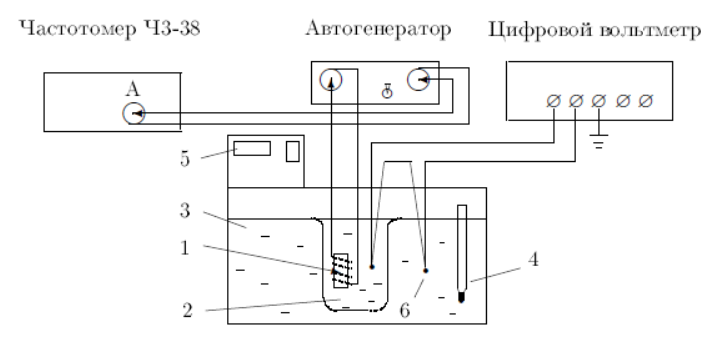
\includegraphics[scale=1]{lab342ris1.png}}
    \caption{\textit{Схема экспериментальной установки}}
\end{figure}

Исследуемый ферромагнитный образец -- в нашем случае гадолиний -- располагается внутри пустотелой катушки самоиндукции входящей в состав LC-автогенератора, который собран на полевом транзисторе КП-103 и выделен в отдельный блок. 

Ввиду хорошей проводимости гадолиния и высокой рабочей частоты генератора ($\sim$ 50кГц) образец изготавливается из мелких кусочков размером около 0,5мм -- для уменьшения вихревых потоков. Катушка 1 с образцом помещена в стеклянный сосуд 2, залитый трансформаторным маслом, которое призвано улучшить тепловой контакт между образцом и термостатируемой жидкостью 3. В емкость вмонитрован термометр 4.

Обозначив за $L$ самоиндукцию катушки с образцом и через $L_0$ -- самоиндукцию в отсутствиие образца, получим:

\begin{equation}
    (L-L_0) \sim \chi.    
\end{equation}

По формуле Томсона период колебаний автогенератора с емкостью контура автогенератора C:

\begin{equation}
    \tau = 2 \pi \sqrt{LC}, \,\
    \tau = 2 \pi \sqrt{L_0C}.
\end{equation}

Тогда из (4) получаем:

\begin{equation}
    (L - L_0) \sim (\tau^2 - \tau_0^2) \longrightarrow \chi \sim (\tau^2 - \tau_0^2).
\end{equation}

Тогда получаем, что закон Кюри-Вейсса справедлив, если выполнено соотношение:

\begin{equation}
    \frac{1}{\chi} \sim (T - \theta_p) \sim \frac{1}{(\tau^2 - \tau_0^2)}.
\end{equation}

Величина стабилизирующей температуры задаётся на дисплее 5 термостата. Для нагрева служит внутренний электронагреватель, для охлаждения циркуллирующая водопроводная вода. 

\subsection*{Ход работы}

Подготовим приборы к работе. Оценим допустимую ЭДС термопары, если допустимая разность температур образца и рабочей жидкости $\Delta T = 0,5 ^\circ C$, а постоянная термопары $k = 24 \, град/мВ$.

Исследуем зависимость периода колебаний LC - генератора от температуры образца, отмечая период колебаний $\tau$ по частотомеру, а температуру T -- по показаниям дисплея и цифровому вольтметру. Проведем измерения в диапазоне от $14 ^\circ C$ до $40 ^\circ C$ через $2 ^\circ C$. Результаты отразим в таблице 1.

\subsection*{Обработка результатов}



\end{document}

